\documentclass[10pt, a4paper]{beamer} %handout fuer eine gedruckte version der slides
\usetheme{metropolis}
\usepackage{polyglossia}
\setmainlanguage{english}

\usepackage{listings,xcolor}
\usepackage{graphicx}

\usepackage{fontspec}
% \setmainfont{UbuntuMono}
\newfontfamily\Bera{Bitstream Vera Sans Mono}[Scale=0.85]

\definecolor{mDarkTeal}{HTML}{23373b}
\definecolor{mLightBrown}{HTML}{EB811B}


\definecolor{lstgrey}{rgb}{0.95,0.95,0.95}
\lstset{language=C,
    backgroundcolor=\color{lstgrey},
    frame=single,
    rulecolor=\color{lstgrey}, % make frame "invisible"
    basicstyle=\Bera\tiny,
    keywordstyle=\bfseries,
    commentstyle=\itshape,
    captionpos=t,
    tabsize=2,
    numberbychapter=false,
    showstringspaces=false,
    breaklines=true,
    morekeywords={public, class, int, return,include}
}
%


\setbeamertemplate{section in toc}{%
  {\color{mDarkTeal}\rule[0.3ex]{3pt}{3pt}}~\inserttocsection\par}
\setbeamertemplate{subsection in toc}{%
  \hspace{1.2em}{\color{mLightBrown}\rule[0.3ex]{3pt}{3pt}}~\inserttocsubsection\par}


% \usecolortheme{spruce}
\AtBeginSection[]
{
  \begin{frame}
    \frametitle{Table of Contents}
    \tableofcontents[currentsection]
  \end{frame}
}

\title[Crisis] % (optional, only for long titles)
{Foundations of Programming in Python}
\author % (optional, for multiple authors)
{Philipp Gloor\inst{1}}
\institute
{
  \inst{1}%
  University of Zurich
}
\date{}
\subject{Python}

\begin{document}
\begin{frame}
\titlepage
\end{frame}

\begin{frame}
\frametitle{About me}

\begin{block}{Education}
    \begin{itemize}
        \item 2012 -- Bachelor of Science UZH in Physics
        \item 2016 -- Master of Science UZH in Computational Science
    \end{itemize}
\end{block}

\begin{block}{Work}
    \begin{itemize}
        \item 2012 -- 2016 Software engineer CERN (remote)
        \item 2016 -- now PDF Tools AG
    \end{itemize}
\end{block}

\begin{block}{Programming experience}
    \begin{itemize}
        \item[] C++, C\#, Java, JavaScript, Python
    \end{itemize}
\end{block}

\begin{block}{Email}
\begin{itemize}
    \item[] philipp.gloor@gmail.com
\end{itemize}
    
\end{block}
 
% In this slide, some important text will be
% \alert{highlighted} beause it's important.
% Please, don't abuse it.
 
% \begin{block}{Remark}
% Sample text
% \end{block}
 
% \begin{alertblock}{Important theorem}
% Sample text in red box
% \end{alertblock}
 
% \begin{examples}
% Sample text in green box. "Examples" is fixed as block title.
% \end{examples}
\end{frame}
\begin{frame}[t]\frametitle{Round of introduction}
    \begin{itemize}
        \item Name
        \item Occupation
        \item Programming experience? What language?
        \item Expectations
    \end{itemize}
\end{frame}

\begin{frame}[t]\frametitle{Learning targets}
    
After this course...
\begin{itemize}
    \item ... you will know what programming is
    \item ... you will know how to write a basic computer program
    \item ... you will know the fundamental components of programming
    \item ... you are able to run Python code
    \item ... you are able to write a Python program based on a written out
    problem statement
    \item ... you know where you can find more information to improve your
    programming skills
\end{itemize}
\end{frame}


\begin{frame}[t]\frametitle{Table of Contents}
    \tableofcontents
\end{frame}

\section{Introduction to Programming} % (fold)
\label{sec:introduction_to_programming}

\begin{frame}[c]\frametitle{Introduction to Programming}
\begin{block}{Modular System}
    \begin{itemize}
        \item \textbf{Input}: Data input from keyboard, files, internet, etc...
        \item \textbf{Output}: Processed data is displayed or saved to a file
        \item \textbf{Assignment}: Values are assigned to variables
        \item \textbf{Conditional execution}: Statements are executed only if certain
        conditions are fulfilled
        \item \textbf{Loops}: Repeating statement or group of statements
        \item \textbf{Libraries}: Using existing implementations
    \end{itemize}

\end{block}     
\end{frame}

\begin{frame}[fragile,c]\frametitle{Examples: Hello World}
    \begin{block}{Java}
    \begin{lstlisting}
        public class HelloWorld {
            public static void main(String args[]) {
                System.out.println("Hello World");
            }
        }
    \end{lstlisting}    
    \end{block}
    
    \begin{block}{C++}
    \begin{lstlisting}
        #include <iostream>
        int main() {
            std::cout << "Hello World" << std::endl;
            return 0;
        }
    \end{lstlisting}    
    \end{block}
    
    \begin{block}{Python}
        \begin{lstlisting}
            print("Hello World")
        \end{lstlisting}
    \end{block}
    
\end{frame}

\begin{frame}[c]\frametitle{Why Python?}
    \begin{columns}
        \begin{column}{0.5\textwidth}
           \begin{itemize}
                \item "Simple" syntax
                \item High-level programming language
                \item Cross-platform
                \item Interpreted
                \item Object-oriented
                \item Many libraries available
            \end{itemize}
        \end{column}
        \begin{column}{0.5\textwidth}  %%<--- here
            \begin{figure}
                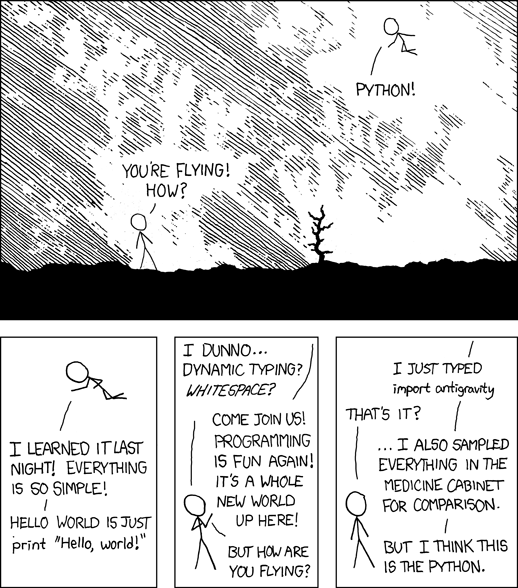
\includegraphics[width=0.9\linewidth]{pics/python.png}
            \end{figure}
        \end{column}
    \end{columns}

\end{frame}
% section introduction_to_programming (end)

\section{Fundamental Concepts} % (fold)
\label{sec:fundamental_concepts}

\subsection{Values, Variables, Expressions, Operators, Comments} % (fold)
\label{sub:values_variables_expressions_operators_comments}

% subsection values_variables_expressions_operators_comments (end)

\subsection{Functions} % (fold)
\label{sub:functions}

% subsection functions (end)

\subsection{Conditionals} % (fold)
\label{sub:conditionals}

% subsection conditionals (end)

\subsection{Functions with Return Values} % (fold)
\label{sub:functions_with_return_values}

% subsection functions_with_return_values (end)

\subsection{Lists} % (fold)
\label{sub:lists}

% subsection lists (end)

\subsection{Iteration} % (fold)
\label{sub:iteration}

% subsection iteration (end)

\subsection{Dictionaries} % (fold)
\label{sub:dictionaries}

% subsection dictionaries (end)
% section fundamental_concepts (end)

\section{Persistence} % (fold)
\label{sec:persistence}

% section persistence (end)

\end{document}
